\chapter{Evaluation}
\label{ch:evaluation}

\begin{figure}
	\begin{center}
		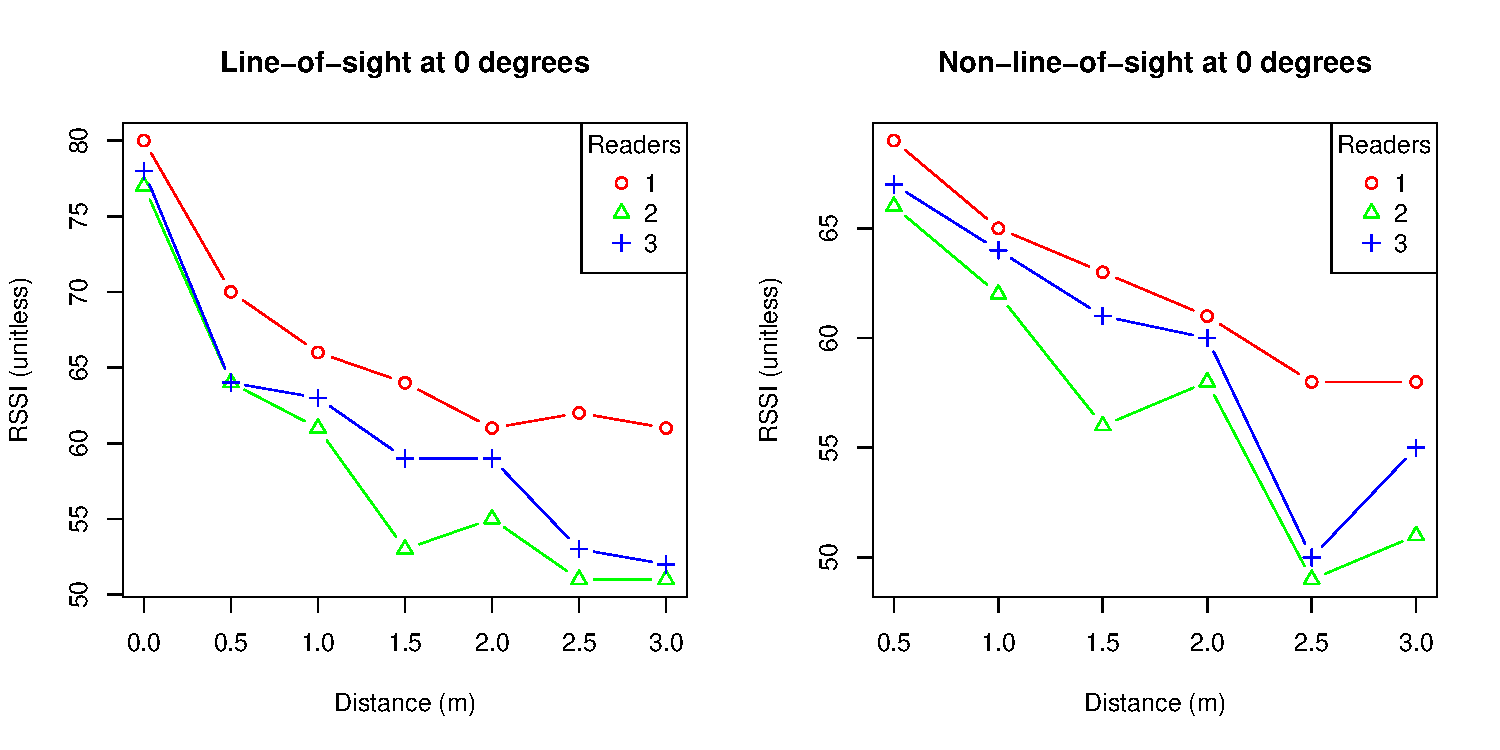
\includegraphics[width=1\textwidth]{figures/rssi_distance_3m_0deg}
		\caption{Two plots of RSSI measurements at increasing distances with the readers at 0 degrees (antennas facing the tag). The left graph show how RSSI values change with a line-of-sight signal propagation. The right graph illustrates the same experiment but with a non-line-of-sight signal propagation (there is an obstacle between the reader and the tag).}
	\end{center}
\end{figure}
\begin{figure}
	\begin{center}
		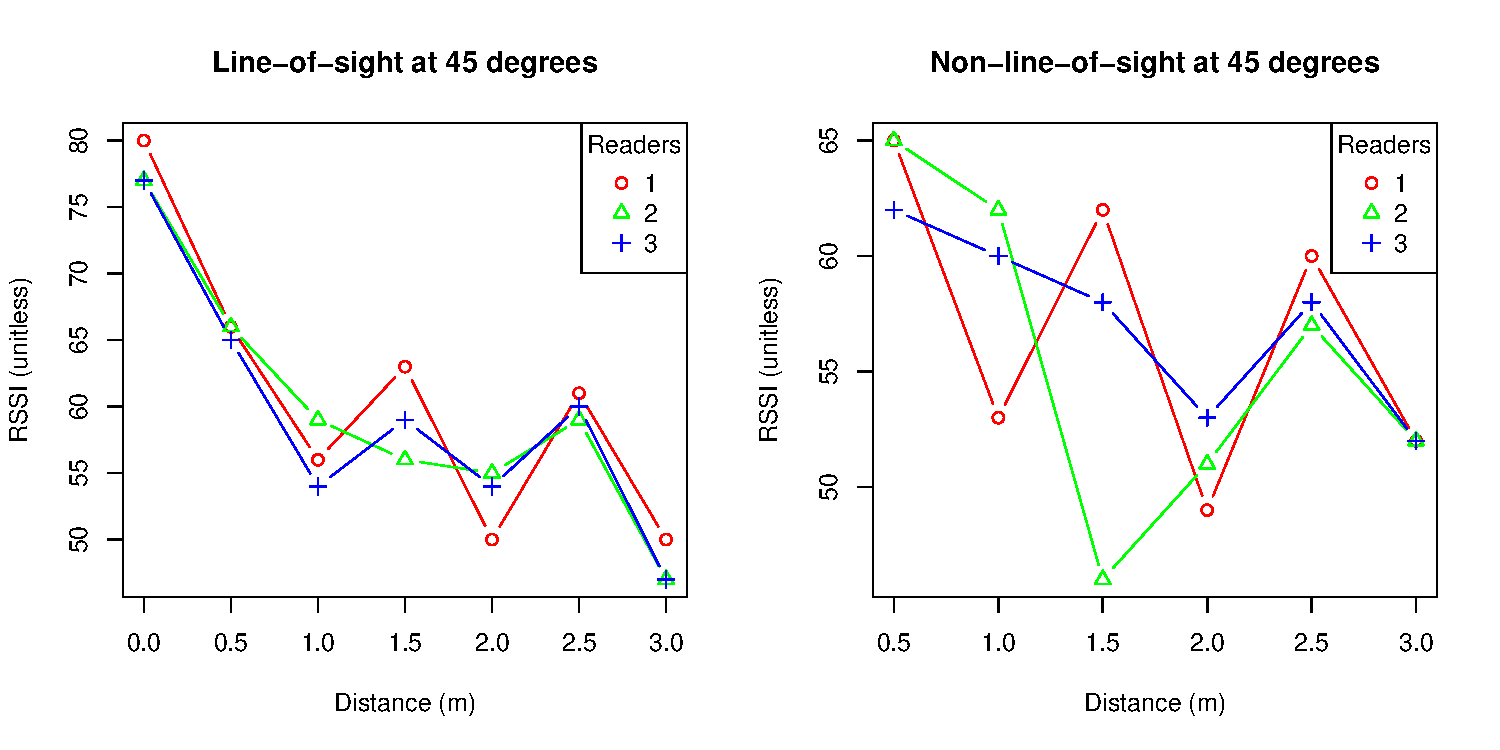
\includegraphics[width=1\textwidth]{figures/rssi_distance_3m_45deg}
		\caption{Two plots of RSSI measurements at increasing distances with the readers at 45 degrees (antennas at an angle to the tag). The left graph show how RSSI values change with a line-of-sight signal propagation. The right graph illustrates the same experiment but with a non-line-of-sight signal propagation (there is an obstacle between the reader and the tag).}
	\end{center}
\end{figure}
\begin{figure}
	\begin{center}
		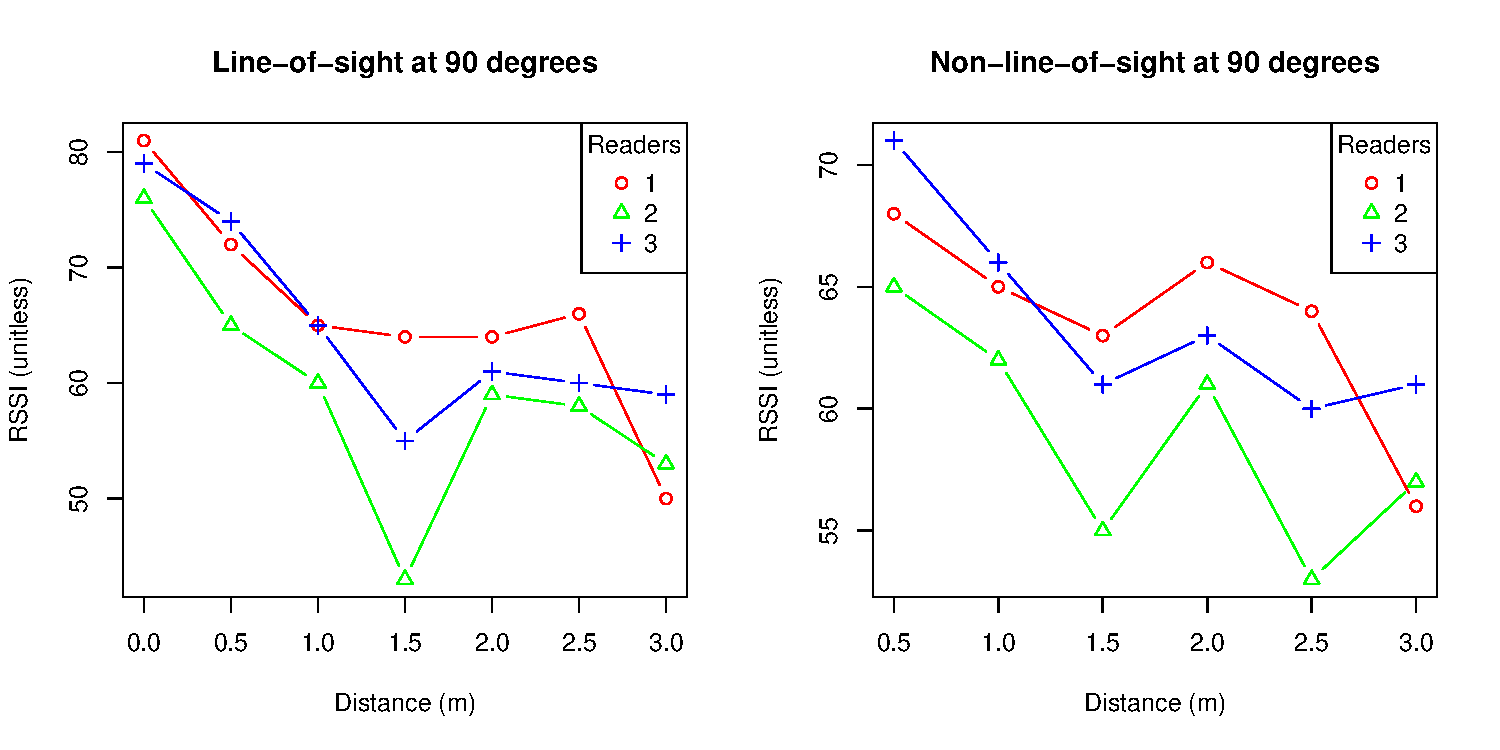
\includegraphics[width=1\textwidth]{figures/rssi_distance_3m_90deg}
		\caption{Two plots of RSSI measurements at increasing distances with the readers at 90 degrees (antennas at an angle to the tag). The left graph show how RSSI values change with a line-of-sight signal propagation. The right graph illustrates the same experiment but with a non-line-of-sight signal propagation (there is an obstacle between the reader and the tag).}
	\end{center}
\end{figure}
\begin{figure}
	\begin{center}
		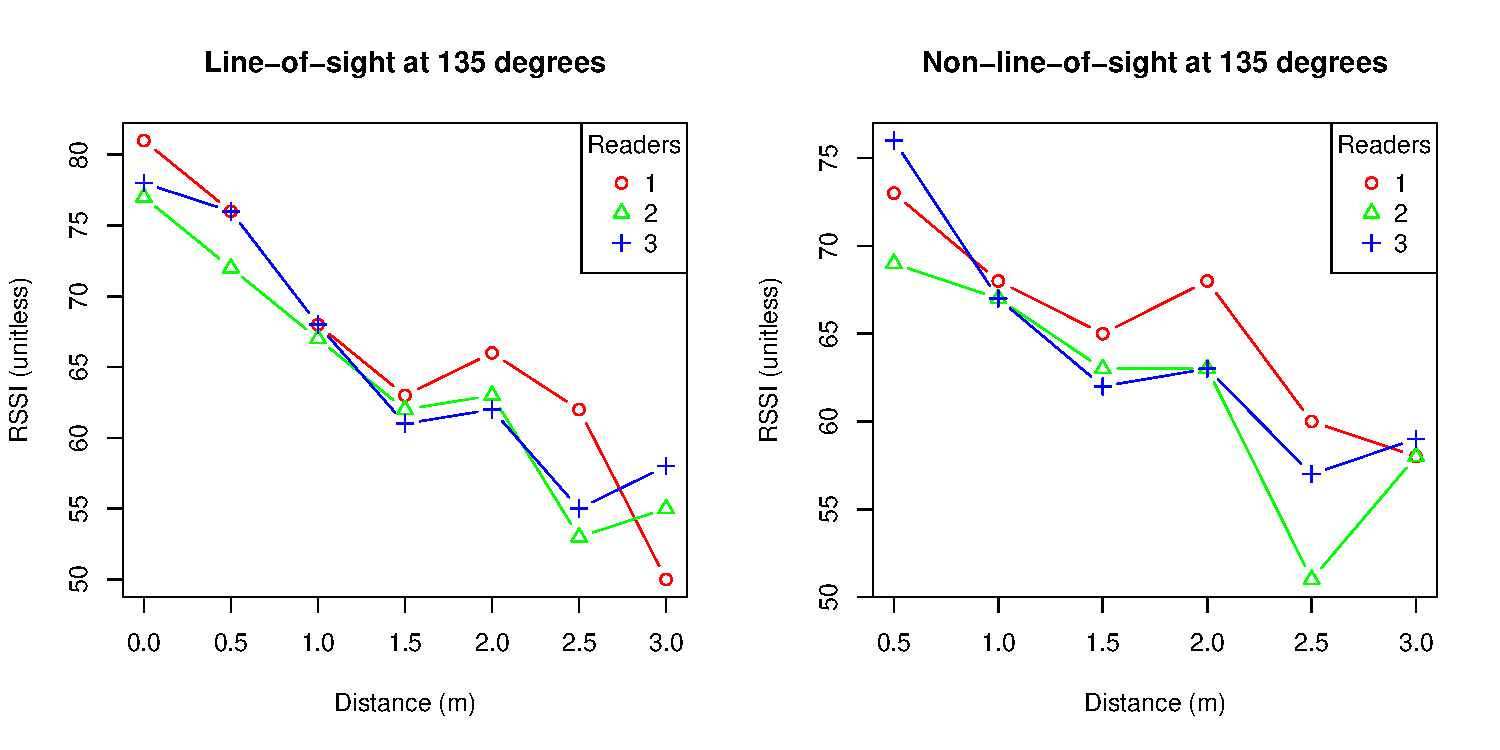
\includegraphics[width=1\textwidth]{figures/rssi_distance_3m_135deg}
		\caption{Two plots of RSSI measurements at increasing distances with the readers at 135 degrees (antennas at an angle to the tag). The left graph show how RSSI values change with a line-of-sight signal propagation. The right graph illustrates the same experiment but with a non-line-of-sight signal propagation (there is an obstacle between the reader and the tag).}
	\end{center}
\end{figure}
\begin{figure}
	\begin{center}
		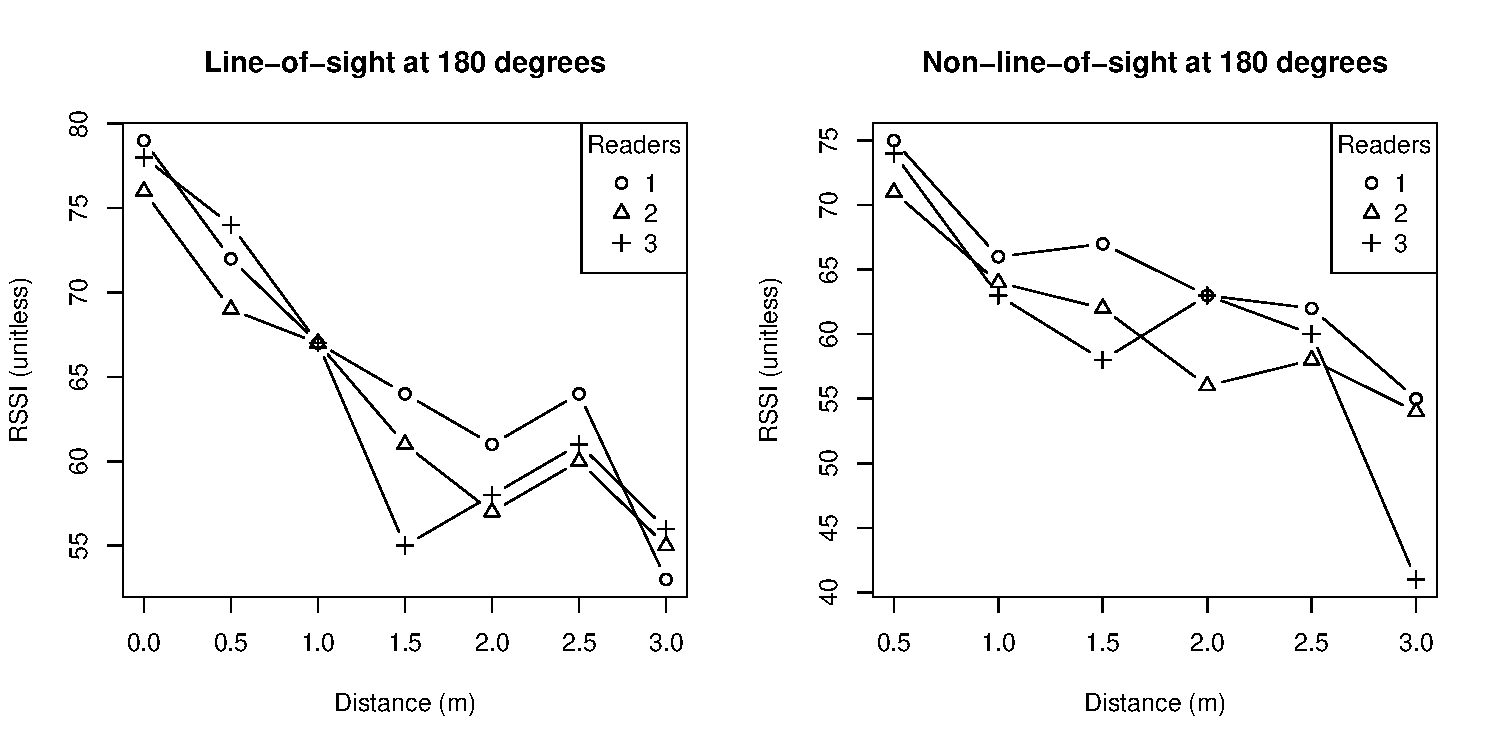
\includegraphics[width=1\textwidth]{figures/rssi_distance_3m_180deg}
		\caption{Two plots of RSSI measurements at increasing distances with the readers at 180 degrees (antennas at an angle to the tag). The left graph show how RSSI values change with a line-of-sight signal propagation. The right graph illustrates the same experiment but with a non-line-of-sight signal propagation (there is an obstacle between the reader and the tag).}
	\end{center}
\end{figure}
\begin{figure}
	\begin{center}
		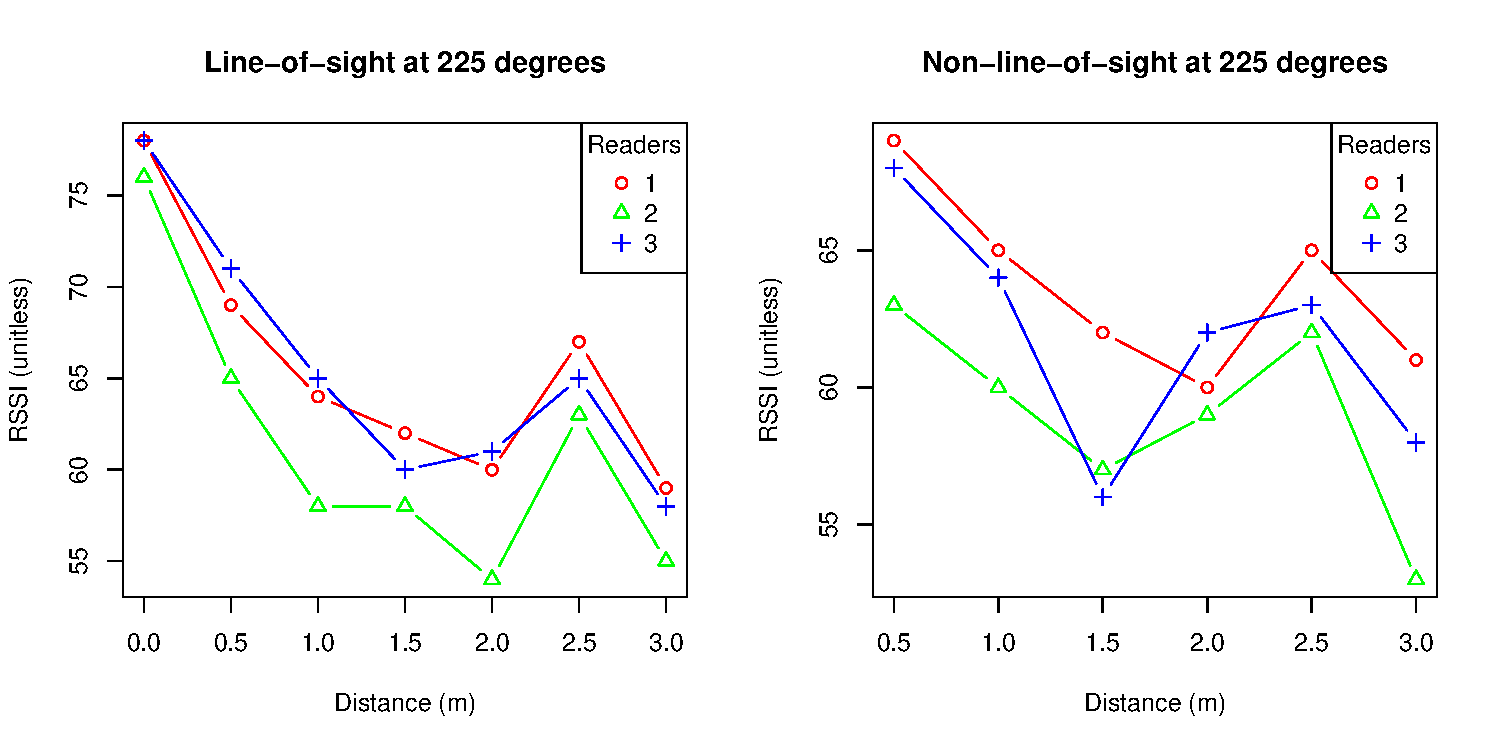
\includegraphics[width=1\textwidth]{figures/rssi_distance_3m_225deg}
		\caption{Two plots of RSSI measurements at increasing distances with the readers at 225 degrees (antennas at an angle to the tag). The left graph show how RSSI values change with a line-of-sight signal propagation. The right graph illustrates the same experiment but with a non-line-of-sight signal propagation (there is an obstacle between the reader and the tag).}
	\end{center}
\end{figure}
\begin{figure}
	\begin{center}
		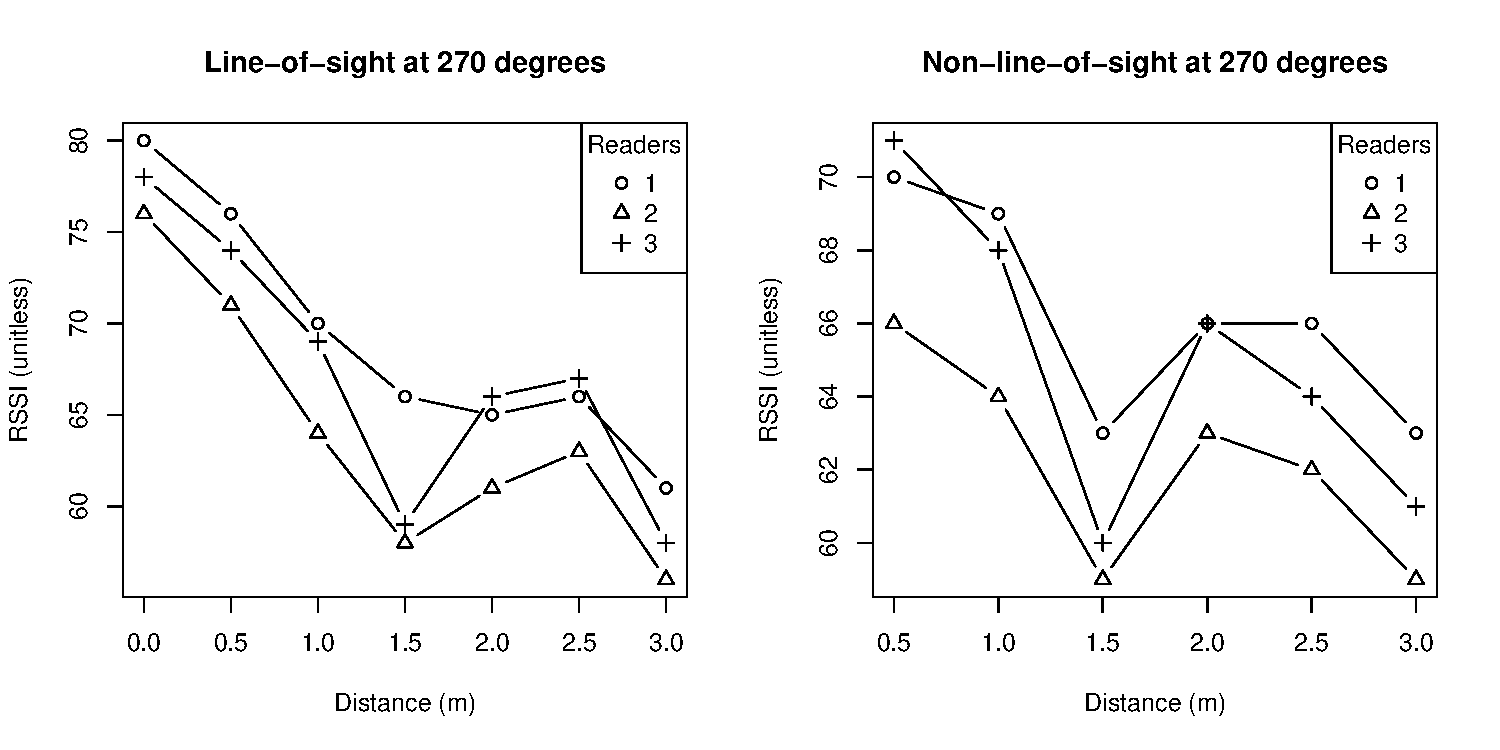
\includegraphics[width=1\textwidth]{figures/rssi_distance_3m_270deg}
		\caption{Two plots of RSSI measurements at increasing distances with the readers at 270 degrees (antennas at an angle to the tag). The left graph show how RSSI values change with a line-of-sight signal propagation. The right graph illustrates the same experiment but with a non-line-of-sight signal propagation (there is an obstacle between the reader and the tag).}
	\end{center}
\end{figure}
\begin{figure}
	\begin{center}
		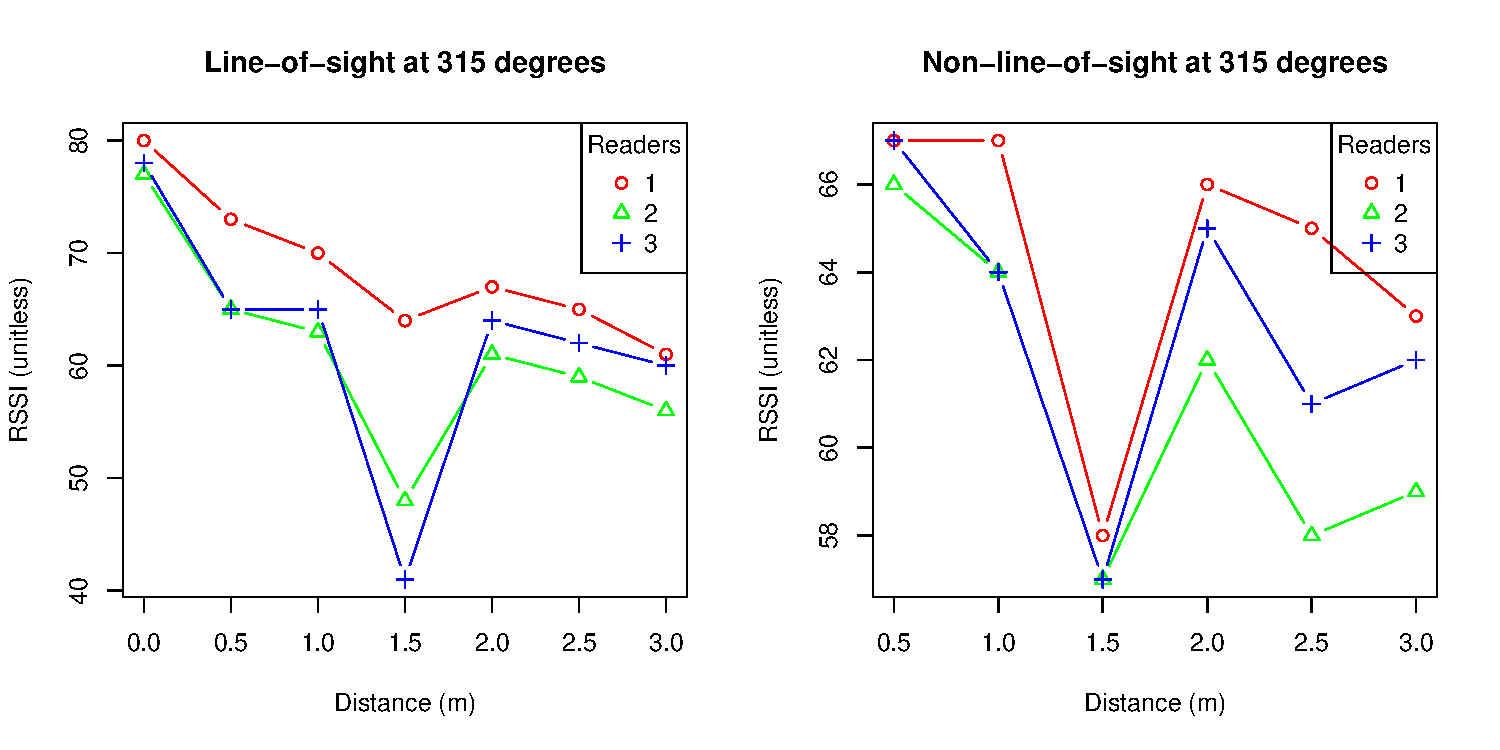
\includegraphics[width=1\textwidth]{figures/rssi_distance_3m_315deg}
		\caption{Two plots of RSSI measurements at increasing distances with the readers at 315 degrees (antennas at an angle to the tag). The left graph show how RSSI values change with a line-of-sight signal propagation. The right graph illustrates the same experiment but with a non-line-of-sight signal propagation (there is an obstacle between the reader and the tag).}
	\end{center}
\end{figure}
\begin{figure}
	\begin{center}
		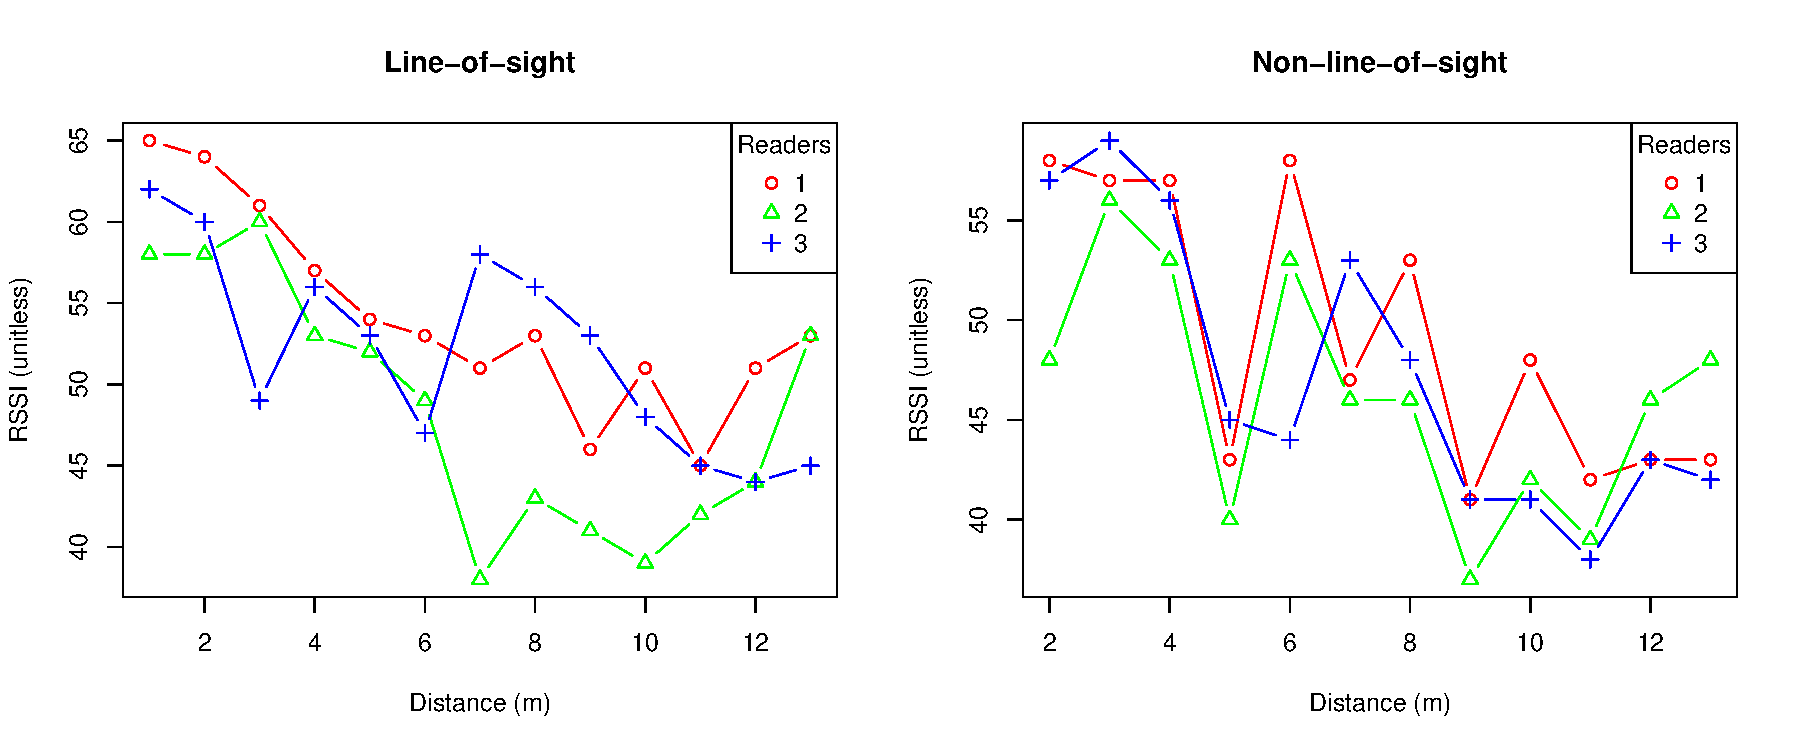
\includegraphics[width=1\textwidth]{figures/rssi_distance_13m}
		\caption{Two plots of RSSI measurements at increasing distances with the readers facing the tag. The left graph show how RSSI values change with a line-of-sight signal propagation. The right graph illustrates the same experiment but with a non-line-of-sight signal propagation (there is an obstacle between the reader and the tag).}
	\end{center}
\end{figure}
\begin{figure}
	\begin{center}
		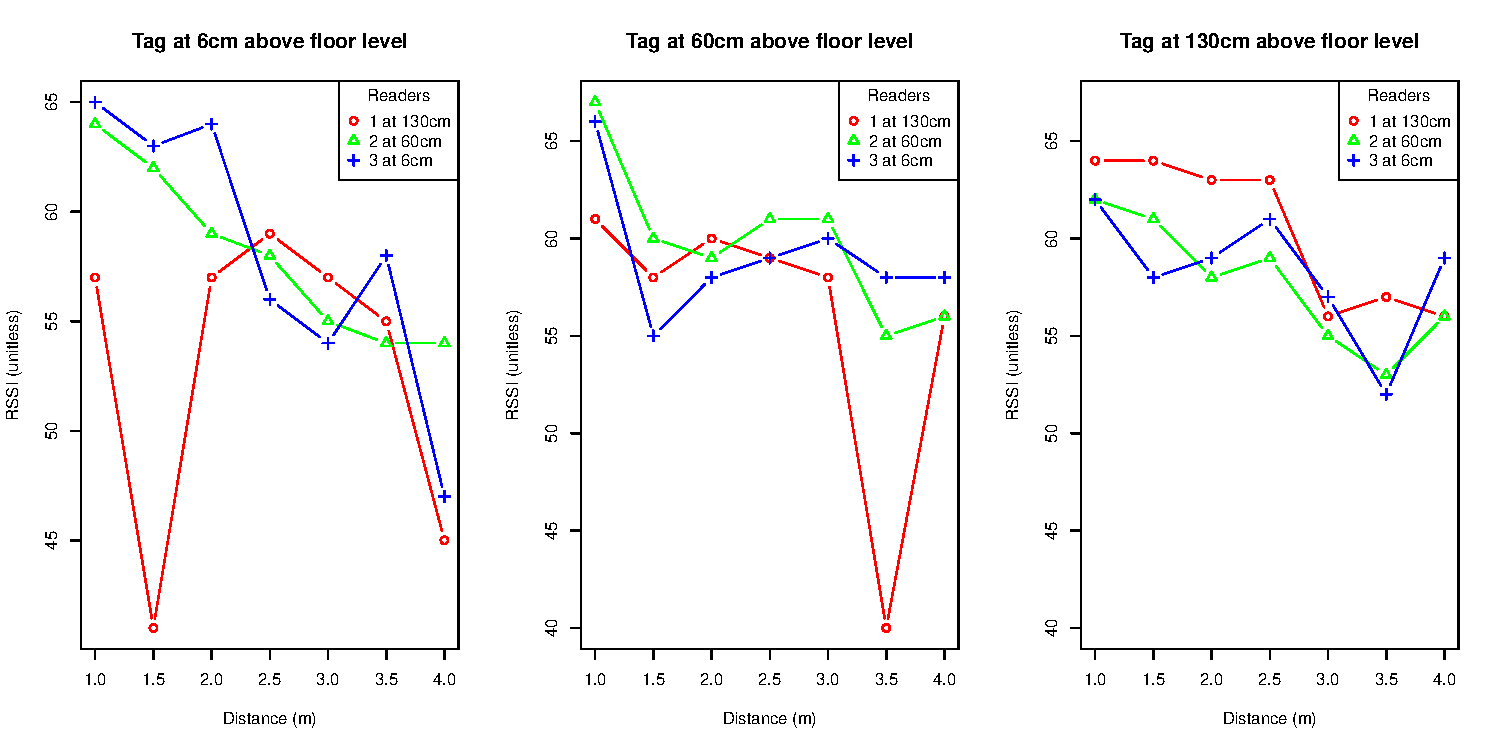
\includegraphics[width=1\textwidth]{figures/rssi_distance_4m}
		\caption{Three plots of RSSI measurements at increasing distances with the readers at different elevation from the floor in an indoor environment. The first graph shows how RSSI measurements change as the distance grows when the tag is placed at 6cm above floor level. The second and third graph show the same experiment but the tag is at 60cm and 130cm above the floor level.}
	\end{center}
\end{figure}
\begin{figure}
	\begin{center}
		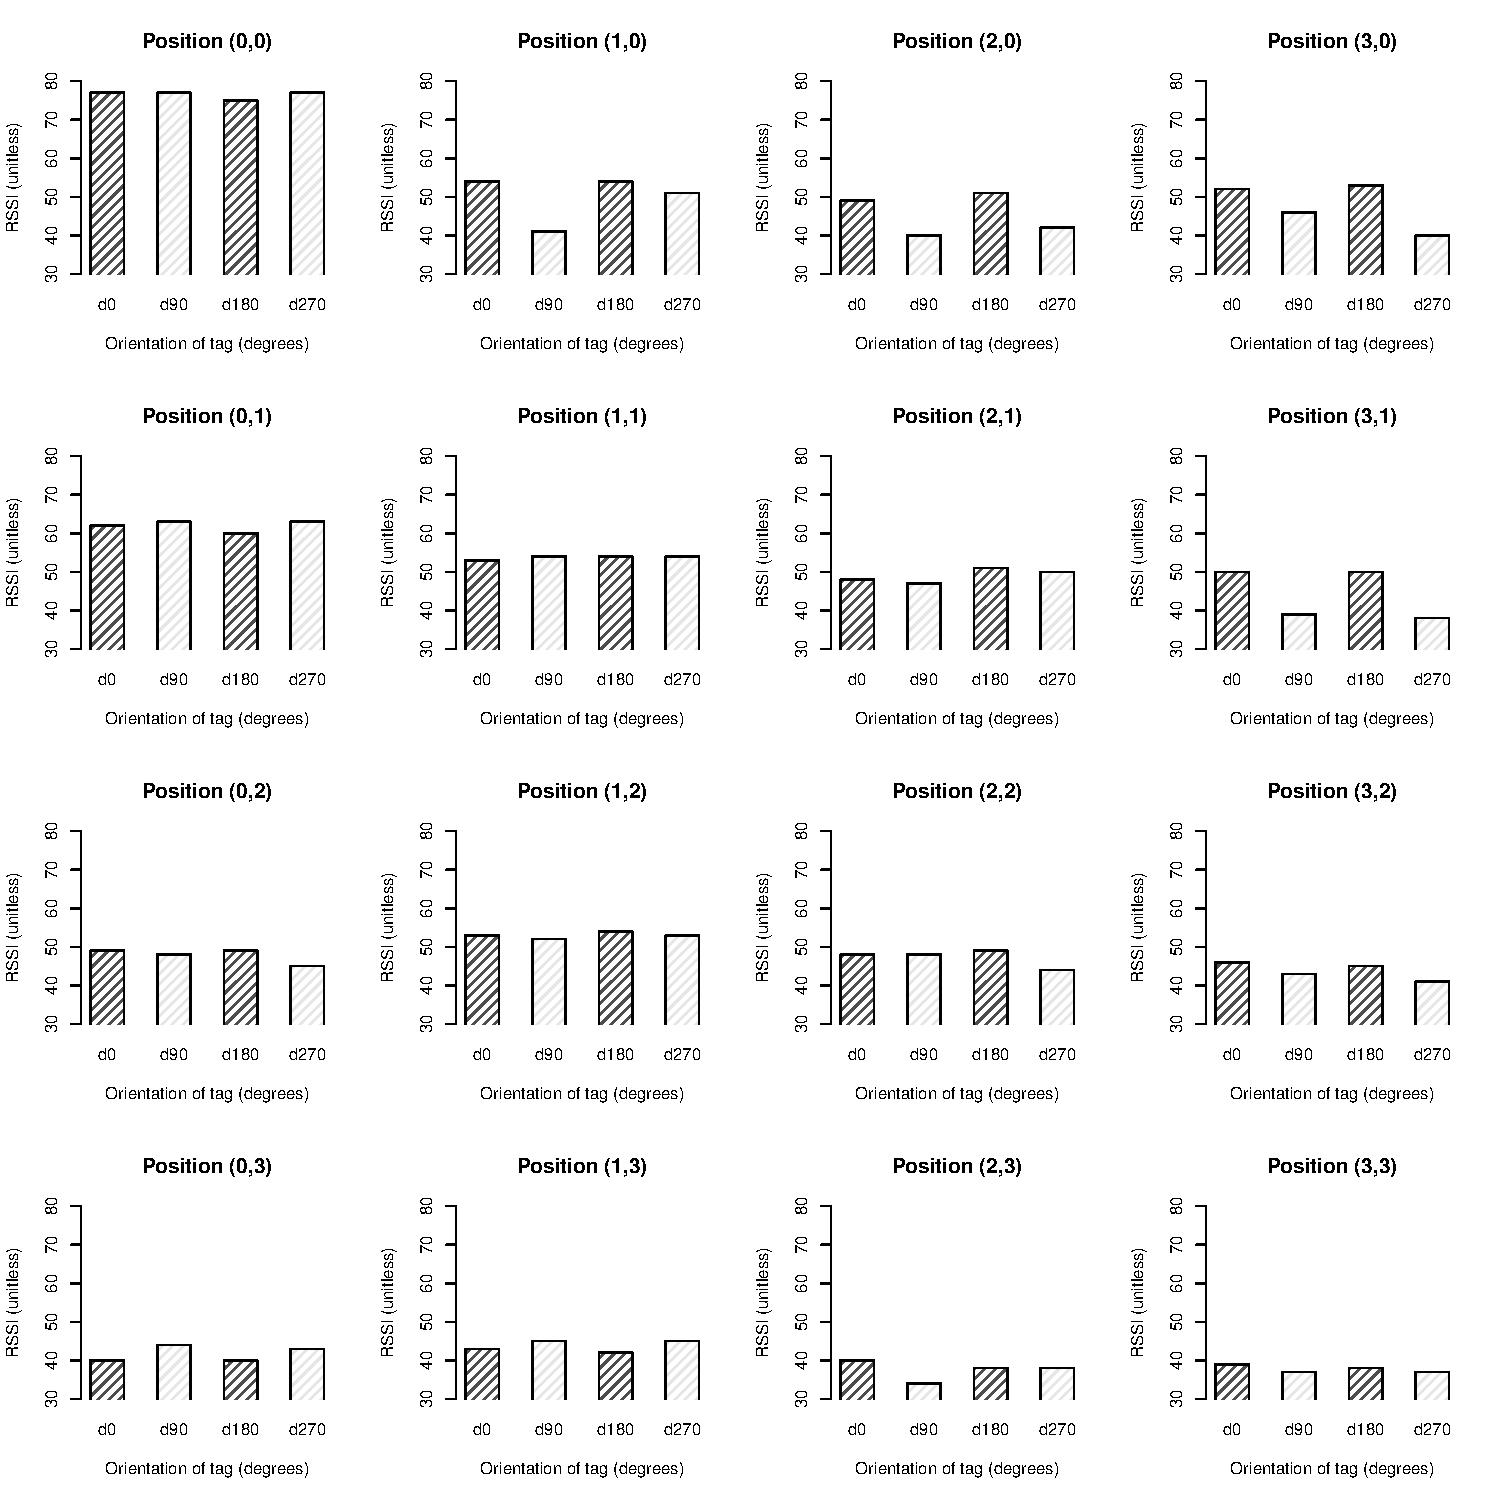
\includegraphics[width=1\textwidth]{figures/rssi_distance_grid_r1}
		\caption{Sixteen plots are organised into a four by four grid. Each plot represents the RSSI measurements of the \textbf{first} reader when the tag is placed at different positions on the x and y axes of the grid. The positions of the tag are all measured in meters. Every four bars in each plot show the RSSI readings when the tag is facing right (0\textdegree), up(90\textdegree), left (180\textdegree), and down (270\textdegree).}
	\end{center}
\end{figure}
\begin{figure}
	\begin{center}
		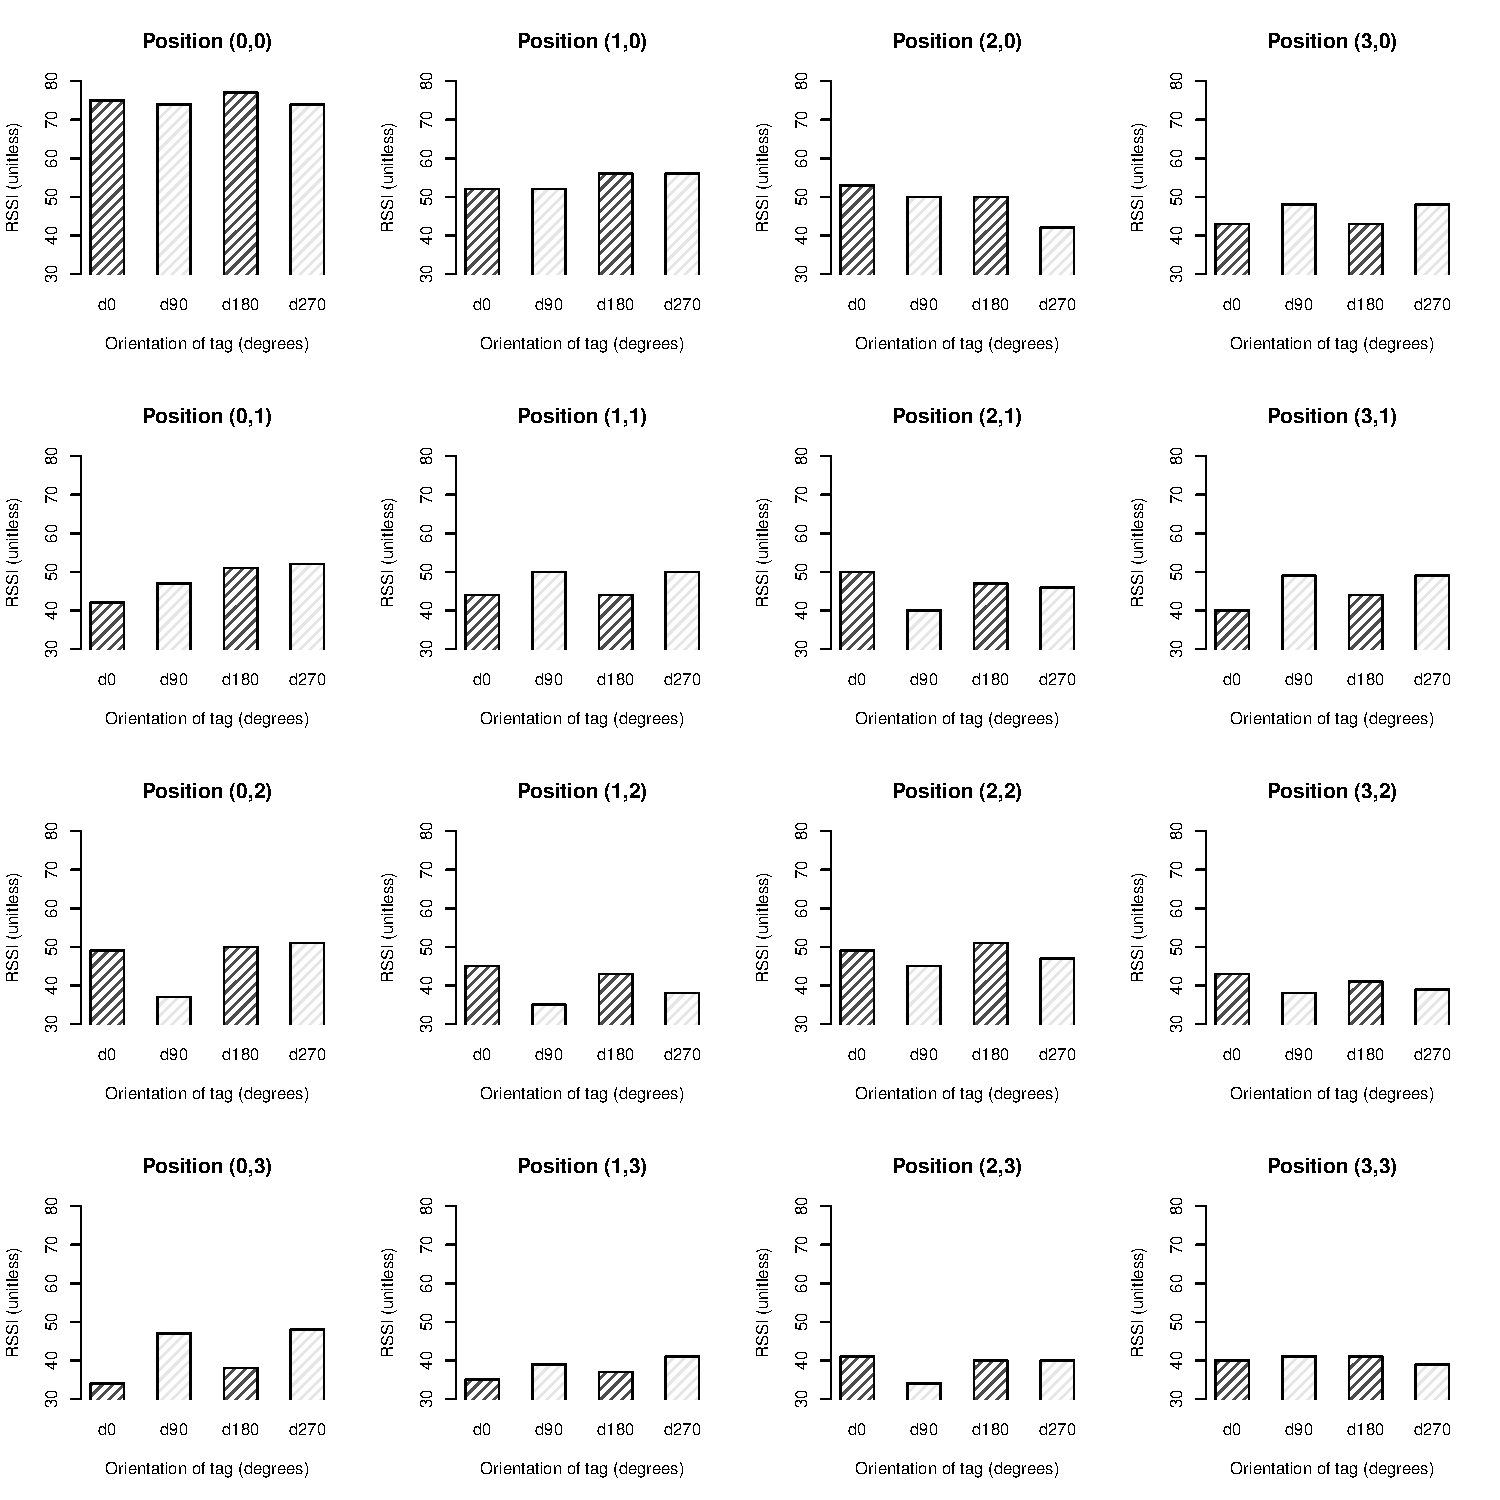
\includegraphics[width=1\textwidth]{figures/rssi_distance_grid_r2}
		\caption{Sixteen plots are organised into a four by four grid. Each plot represents the RSSI measurements of the \textbf{second} reader when the tag is placed at different positions on the x and y axes of the grid. The positions of the tag are all measured in meters. Every four bars in each plot show the RSSI readings when the tag is facing right (0\textdegree), up(90\textdegree), left (180\textdegree), and down (270\textdegree).}
	\end{center}
\end{figure}
\begin{figure}
	\begin{center}
		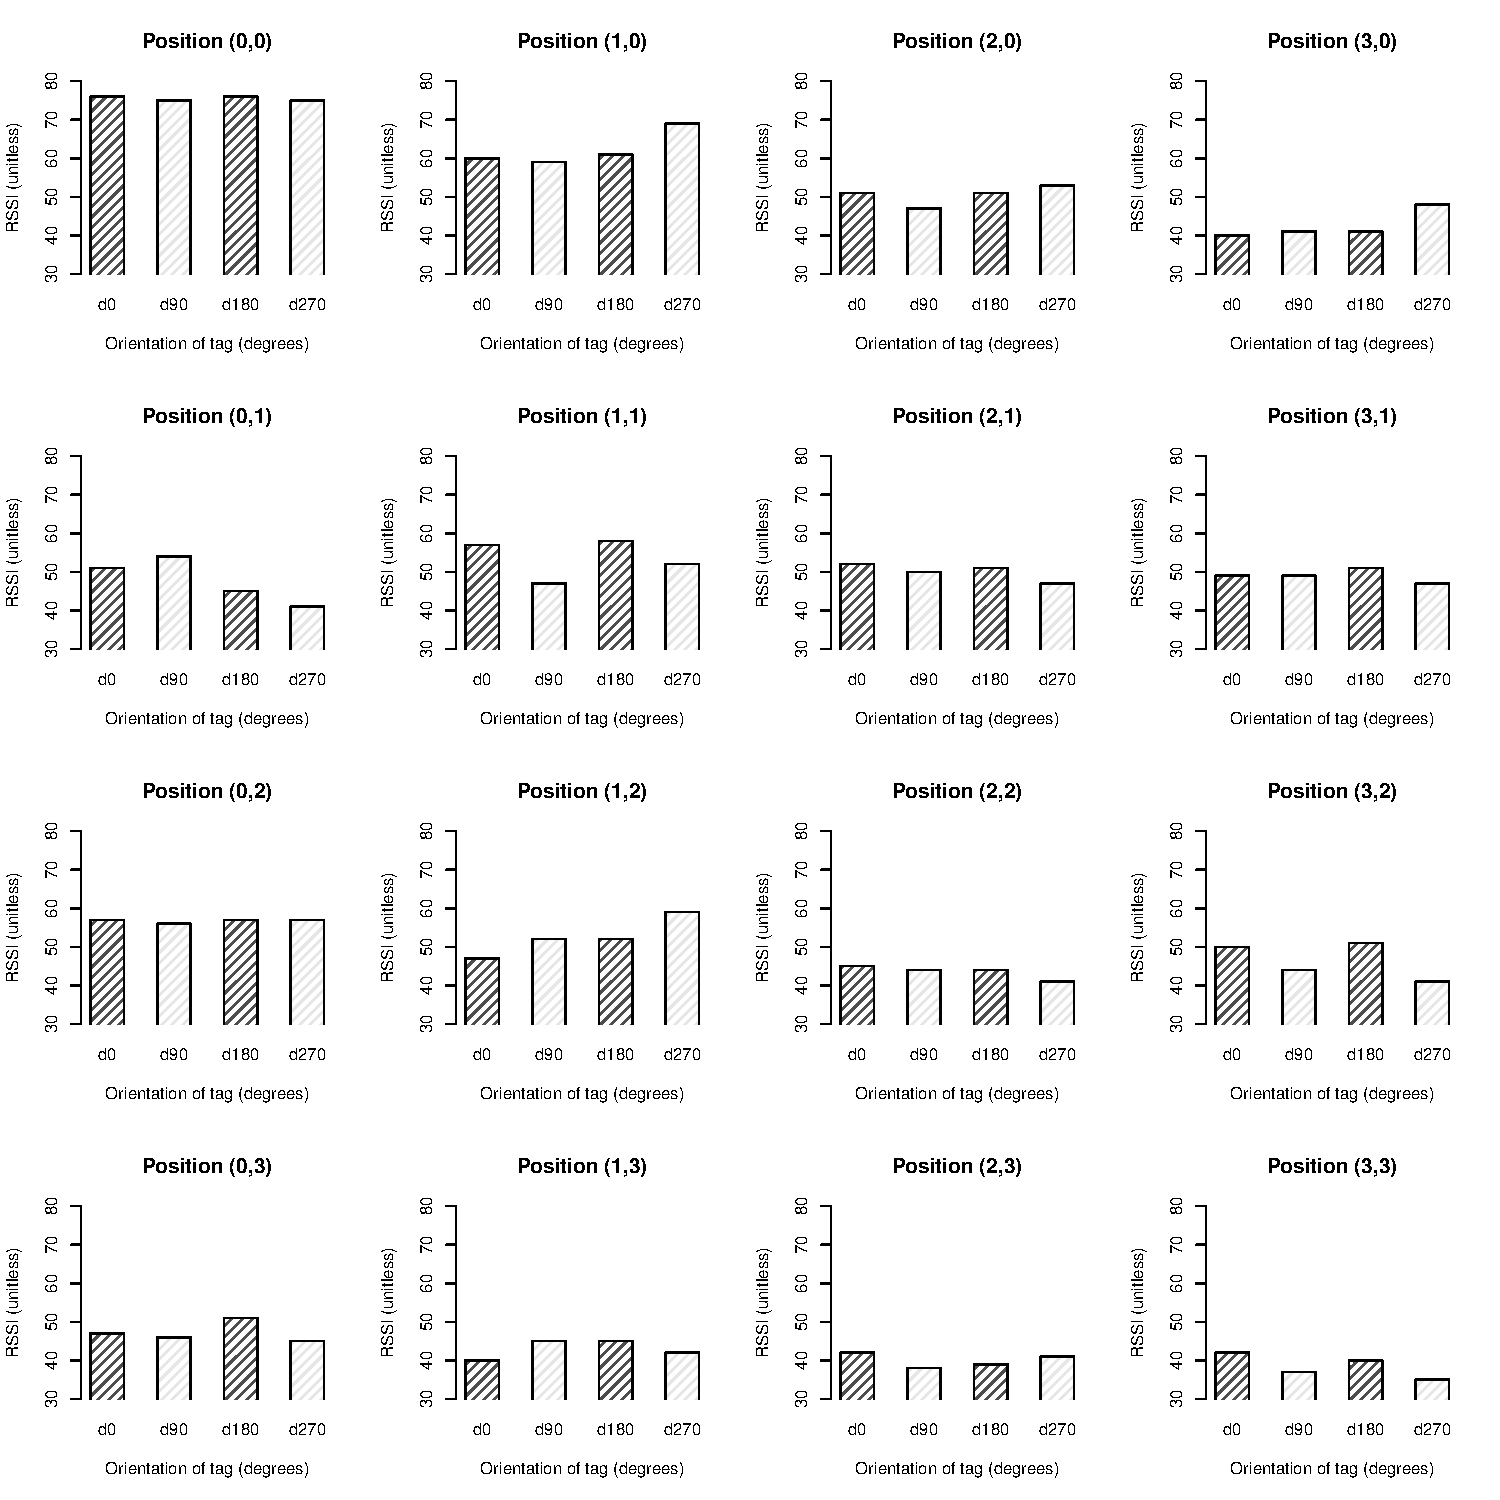
\includegraphics[width=1\textwidth]{figures/rssi_distance_grid_r3}
		\caption{Sixteen plots are organised into a four by four grid. Each plot represents the RSSI measurements of the \textbf{third} reader when the tag is placed at different positions on the x and y axes of the grid. The positions of the tag are all measured in meters. Every four bars in each plot show the RSSI readings when the tag is facing right (0\textdegree), up(90\textdegree), left (180\textdegree), and down (270\textdegree).}
	\end{center}
\end{figure}
\begin{figure}
	\begin{center}
		
\includegraphics[width=1\textwidth]{figures/error_distance_grid}
		\caption{Sixteen plots are organised into a four by four grid. The readers are placed at positions (0,0), (0,3), and (3,0). Each plot represents the error in meters between measured and estimated location when the tag is placed at different positions on the grid. Each plot consists of four ellipses that illustrate the x and y error when the tag is facing right (0\textdegree), up(90\textdegree), left (180\textdegree), and down (270\textdegree). The colours of the ellipses are red, green, blue, and black, respectively.}
	\end{center}
\end{figure}

\begin{figure}
	\begin{center}
		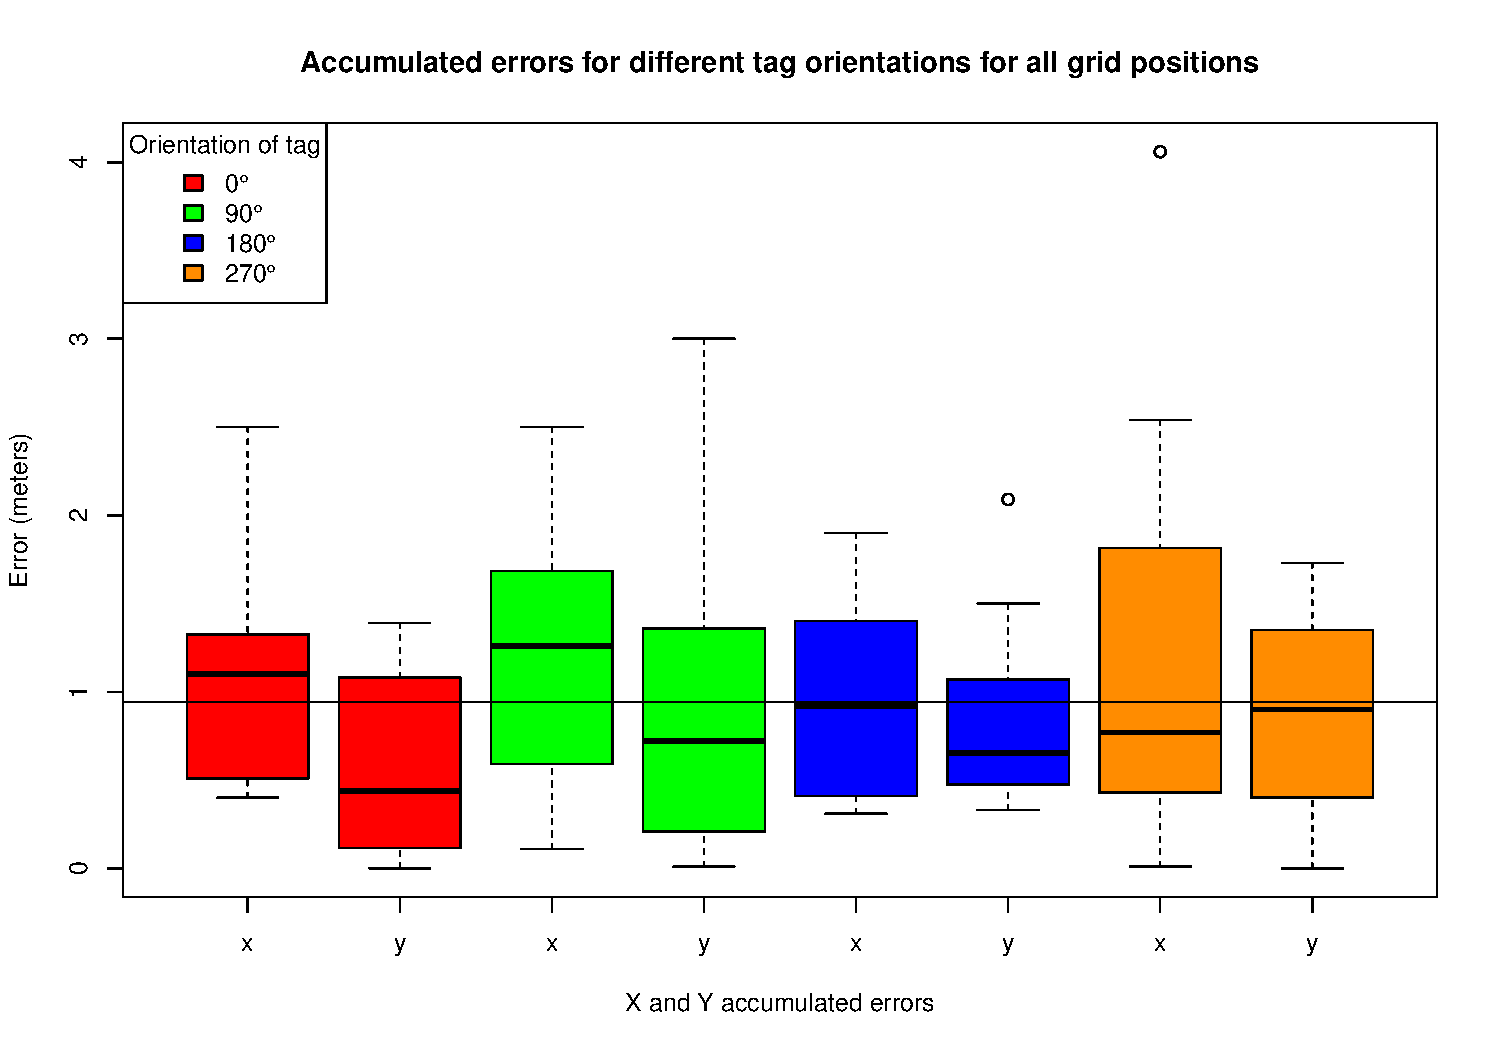
\includegraphics[width=1\textwidth]{figures/error_boxplot}
		\caption{A box plot showing errors between measured and estimated locations. The boxes are organised in four groups. Each group consists of errors in the x and y axes for a particular orientation of the tag. The horizontal line across the plot is the mean of all errors regardless of the tag orientation.}
	\end{center}
\end{figure}

\section{Summary}
